\documentclass{article}

\usepackage{amsmath, amsthm, amssymb, amsfonts}
\usepackage{thmtools}
\usepackage{graphicx}
\usepackage{setspace}
\usepackage{geometry}
\usepackage{float}
\usepackage{hyperref}
\usepackage[utf8]{inputenc}
\usepackage[english]{babel}
\usepackage{framed}
\usepackage[dvipsnames]{xcolor}
\usepackage{tcolorbox}

%Define the listing package
\usepackage{listings} %code highlighter
\usepackage{color} %use color
\definecolor{mygreen}{rgb}{0,0.6,0}
\definecolor{mygray}{rgb}{0.5,0.5,0.5}
\definecolor{mymauve}{rgb}{0.58,0,0.82}
 
%Customize a bit the look
\lstset{ %
backgroundcolor=\color{white}, % choose the background color; you must add \usepackage{color} or \usepackage{xcolor}
basicstyle=\footnotesize, % the size of the fonts that are used for the code
breakatwhitespace=false, % sets if automatic breaks should only happen at whitespace
breaklines=true, % sets automatic line breaking
captionpos=b, % sets the caption-position to bottom
commentstyle=\color{mygreen}, % comment style
deletekeywords={...}, % if you want to delete keywords from the given language
escapeinside={\%*}{*)}, % if you want to add LaTeX within your code
extendedchars=true, % lets you use non-ASCII characters; for 8-bits encodings only, does not work with UTF-8
frame=single, % adds a frame around the code
keepspaces=true, % keeps spaces in text, useful for keeping indentation of code (possibly needs columns=flexible)
keywordstyle=\color{blue}, % keyword style
% language=Octave, % the language of the code
morekeywords={*,...}, % if you want to add more keywords to the set
numbers=left, % where to put the line-numbers; possible values are (none, left, right)
numbersep=5pt, % how far the line-numbers are from the code
numberstyle=\tiny\color{mygray}, % the style that is used for the line-numbers
rulecolor=\color{black}, % if not set, the frame-color may be changed on line-breaks within not-black text (e.g. comments (green here))
showspaces=false, % show spaces everywhere adding particular underscores; it overrides 'showstringspaces'
showstringspaces=false, % underline spaces within strings only
showtabs=false, % show tabs within strings adding particular underscores
stepnumber=1, % the step between two line-numbers. If it's 1, each line will be numbered
stringstyle=\color{mymauve}, % string literal style
tabsize=2, % sets default tabsize to 2 spaces
title=\lstname % show the filename of files included with \lstinputlisting; also try caption instead of title
}
%END of listing package%
 
\definecolor{darkgray}{rgb}{.4,.4,.4}
\definecolor{purple}{rgb}{0.65, 0.12, 0.82}
 
%define Javascript language
\lstdefinelanguage{JavaScript}{
keywords={typeof, new, true, false, catch, function, return, null, catch, switch, var, if, in, while, do, else, case, break},
keywordstyle=\color{blue}\bfseries,
ndkeywords={class, export, boolean, throw, implements, import, this},
ndkeywordstyle=\color{darkgray}\bfseries,
identifierstyle=\color{black},
sensitive=false,
comment=[l]{//},
morecomment=[s]{/*}{*/},
commentstyle=\color{purple}\ttfamily,
stringstyle=\color{red}\ttfamily,
morestring=[b]',
morestring=[b]"
}

\lstset{
language=JavaScript,
extendedchars=true,
basicstyle=\footnotesize\ttfamily,
showstringspaces=false,
showspaces=false,
numbers=left,
numberstyle=\footnotesize,
numbersep=9pt,
tabsize=2,
breaklines=true,
showtabs=false,
captionpos=b
}

\colorlet{LightGray}{White!90!Periwinkle}
\colorlet{LightOrange}{Orange!15}
\colorlet{LightGreen}{Green!15}

\newcommand{\HRule}[1]{\rule{\linewidth}{#1}}

\NewEnviron{NORMAL}{% 
    \scalebox{2}{$\BODY$} 
} 

\declaretheoremstyle[name=Theorem,]{thmsty}
\declaretheorem[style=thmsty,numberwithin=section]{theorem}
\tcolorboxenvironment{theorem}{colback=LightGray}

\declaretheoremstyle[name=Proposition,]{prosty}
\declaretheorem[style=prosty,numberlike=theorem]{proposition}
\tcolorboxenvironment{proposition}{colback=LightOrange}

\declaretheoremstyle[name=Principle,]{prcpsty}
\declaretheorem[style=prcpsty,numberlike=theorem]{principle}
\tcolorboxenvironment{principle}{colback=LightGreen}

\setstretch{1.2}
\geometry{
    textheight=9in,
    textwidth=5.5in,
    top=1in,
    headheight=12pt,
    headsep=25pt,
    footskip=30pt
}

% ------------------------------------------------------------------------------

\begin{document}

% ------------------------------------------------------------------------------
% Cover Page and ToC
% ------------------------------------------------------------------------------

\title{ \normalsize \textsc{}
		\\ [2.0cm]
		\HRule{1.5pt} \\
		\LARGE \textbf{\uppercase{Statistica}
		\HRule{2.0pt} \\ [0.6cm] \LARGE{Corso A} \vspace*{10\baselineskip}}
		}
\date{\text{Ultima Compilazione - }\today}
\author{\textbf{Autore} \\ 
		Giuseppe Acocella \\
		2024/25\\}

\maketitle
\newpage

\tableofcontents

\newpage

\section{Statistica Descrittiva}

Questo ramo della statistica cerca di raccogliere dati per descrivere degli oggetti. Elenchiamo delle definizioni standard:

\begin{enumerate}
    \item \textbf{Popolazione}: Insieme di oggetti da studiare.
    \item \textbf{Carattere}: Caratteristiche degli oggetti della popolazione.
    \begin{enumerate}
        \item Colore di una biglia, altezza di un individuo.
    \end{enumerate}
    Ricordiamo che un carattere può essere sia \textbf{qualitativo} (es. colore) sia \textbf{quantitativo} (es. altezza).
    \item \textbf{Modalità}: Possibili valori che il carattere può assumere.
    \begin{enumerate}
        \item Colore biglia istanziato: rosso, blu. Lancio moneta istanziato: testa/croce.
    \end{enumerate}
    \item \textbf{Campione Statistico (Sample)}: Sottoinsieme della popolazione scelto a rappresentarla.
    \item \textbf{Dati}: Esiti delle misure del carattere sugli individui del campione.
    \begin{enumerate}
        \item Lanci moneta: $T,C,T,T,T,C, \;....$
    \end{enumerate}
    \item \textbf{Taglia Campione}: Numero di elementi nel campione.
\end{enumerate}

\subsection{Frequenze e Campioni}

Abbiamo due tipi di frequenze:

\begin{enumerate}
    \item \textbf{Frequenza Assoluta}: Corrisponde al numero di volte in cui la \textbf{modalità} appare nei \textbf{dati}:
    \[ \#\{\: i \: |\:x_{i} = a \:\} \]
    \item \textbf{Frequenza Relativa}: Corrisponde al numero di volte in cui la \textbf{modalità} appare nei dati fratto il numero dei dati stessi:
    \[ \text{frequenza relativa} = \frac{\text{frequenza assoluta di }a}{\text{taglia campione}} \]
\end{enumerate}

\subsection{Caratteri e Rappresentazioni Grafiche}


La rappresentazione dei dati dipende fortemente dal tipo di \textbf{carattere}:
\vspace*{10px}
\begin{enumerate}
    \item \textbf{Carattere Discreto}: Quantità piccola e finita di modalità assumibili.
    \begin{enumerate}
        \item Lancio di un dado, esiti di un sondaggio.
    \end{enumerate}

\newpage

In questo caso per le rappresentazioni si utilizzano \textbf{diagrammi a barre}.

\begin{figure}[htbp]
    \center
    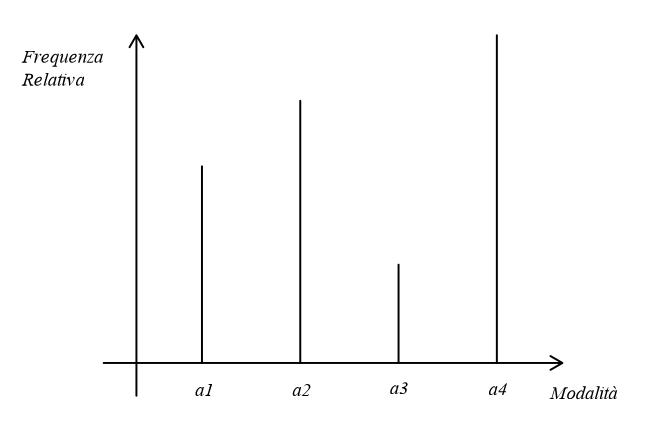
\includegraphics[scale=0.6]{img/diagramma_a_barre.png}
    \caption{Esempio di diagramma a barre.}
\end{figure}

\item \textbf{Carattere Continuo}: Quantità assumibili in un intervallo continuo.
\begin{enumerate}
    \item Altezza della popolazione.
\end{enumerate}

\begin{figure}[htbp]
    \center
    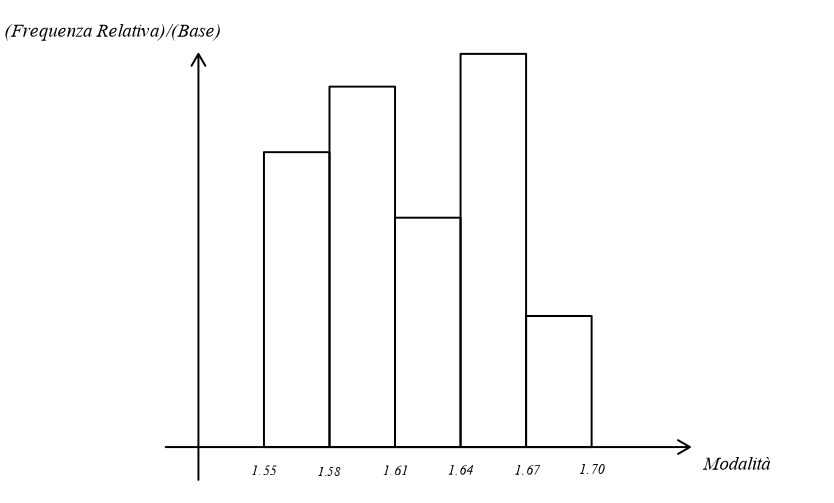
\includegraphics[scale=0.5]{img/istogramma.png}
    \caption{Esempio di istogramma.}
\end{figure}

\vspace*{8px}

La scelta di mettere sull'asse y il rapporto tra freq. relativa e base non è casuale, infatti se scegliessimo intervalli di ampiezza diversa si andrebbe in contro ad un errore di rappresentazione.

\end{enumerate}

\newpage

\subsubsection{Classi di grafici}

Elenchiamo qualche classificazione di rappresentazioni grafiche:

\begin{enumerate}
    \item \textbf{Normale}: Simile ad una campana simmetrica:
    \begin{figure}[htbp]
        \center
        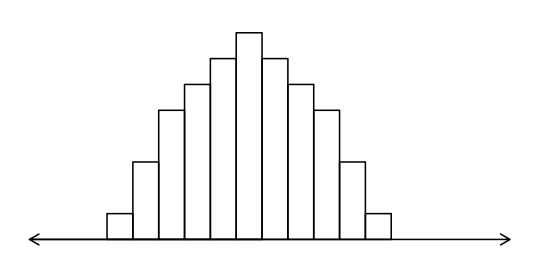
\includegraphics[scale=0.5]{img/normale.png}
    \end{figure}
    \vspace*{8px}

    \item \textbf{Uni/Bi/Tri Modale}: Si concentra attorno ad un numero k di colonne più alte:
    \begin{figure}[htbp]
        \center
        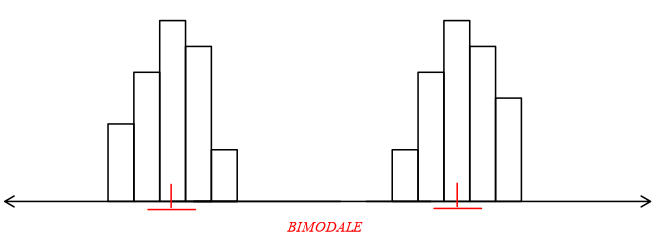
\includegraphics[scale=0.5]{img/modale.png}
    \end{figure}
    \vspace*{8px}

    \begin{enumerate}
        \item \textbf{Modale Asimmetrico Sx/Dx}: Si concentrano attorno ad una colonna più alta in maniera asimmetrica:
        \begin{figure}[H]
  \centering
  \begin{minipage}[b]{0.4\textwidth}
    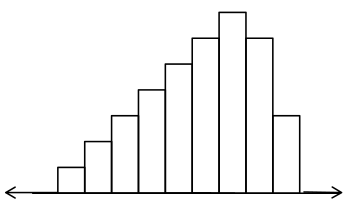
\includegraphics[width=\textwidth]{img/asimmetrico_sx.png}
  \end{minipage}
  \hspace{10px}
  \begin{minipage}[b]{0.4\textwidth}
    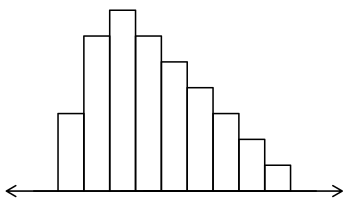
\includegraphics[width=\textwidth]{img/asimmetrico_dx.png}
  \end{minipage}
\end{figure}
    \end{enumerate}
\end{enumerate}

\newpage

\subsection{Indici}

Gli indici statistici sono quantità numeriche che riassumono proprietà significative sulla \textbf{distribuizione dei dati}.

\subsubsection{Indici di Centralità - (Media, Mediana, Moda)}

Descriviamo tre tipi di indici di centralità:

\begin{enumerate}
    \item \textbf{Media Campionaria}: Descriviamo questo indice:
    \[ \overline{x} = \frac{1}{n}\sum_{i=1}^{n} x_{i}\]
    ossia semplicemente la media aritmetica dei dati.
    Un modo \textbf{alternativo} è rappresentarlo così:
    \vspace*{5px}
    \[ \frac{\text{modalita}*\text{frequenza ass. della modalita}}{\text{quantità di dati}} \]
    \vspace*{5px}
    che formalmente si esprime così:
    \[ \overline{x} = \sum_{j=1}^{M}\:a_{j}\:p(a_{j}) \]
    dove $a_{j}$ sta per modalità e $p(a_{j})$ sta per frequenza relativa della modalità.
    \paragraph{Sensibilità ai Valori Estremi} Una delle caratteristiche della media campionaria è quella di essere molto sensibile ai valori estremi del campione.
    \paragraph{Caratteristiche} Riesce a vedere tutti i dati del campione e gode di alcune proprietà matematiche come la linearità.
    \item \textbf{Mediana Campionaria}: Il dato $x_{i}$ sarà \textbf{centrale}, dunque avrà metà dei dati a sinistra e metà a destra. La calcoliamo dunque in due modi:
    \begin{enumerate}
        \item \textbf{Numero dispari di modalità}: Dato centrale.
        \[ \text{mediana} = x(\frac{n+1}{2}) \]
        \item \textbf{Numero pari di modalità}: Media tra i due dati centrali.
        \[ \text{mediana} = \frac{1}{2}(x_{\frac{n}{2}} + x_{\frac{n}{2}+1}) \]
    \end{enumerate}
    \paragraph{Caratteristiche} Più robusta rispetto ai valori estremi.
    \item \textbf{Moda}: Modalità più frequente tra i dati.
\end{enumerate}

\newpage

\subsubsection{Indici di Dispersione - (Varianza, Deviazione Standard)}

Gli indici di dispersione ci permettono di stabilire quanto i valori della distribuzione si allontanino da un valore centrale scelto come riferimento.
Elenchiamoli:

\begin{enumerate}
    \item \textbf{Varianza Campionaria/Empirica}: Permette di 
    \[ \text{CAMPIONARIA:} \:\:\:\: Var(x) = \frac{1}{n-1} \sum^{n}_{i=1}(x_{i}-\overline{x})^{2} \]
    \[ \text{EMPIRICA:} \:\:\:\: Var_{e}(x) = \frac{1}{n} \sum^{n}_{i=1}(x_{i}-\overline{x})^{2} = (\frac{1}{n}\sum^{n}_{i=1}x^{2}_{i}) - \overline{x}^{2}\]
    \vspace*{5px}
    E' possibile calcolare la varianza anche con le frequenze relative:
    \[ Var_{e}(x) = (\:\sum_{j=1}^{M}a^{2}_{j} * p(a_{j})\:) - \overline{x}^{2}\]
    \item \textbf{Scarto Quadratico Medio}: Indice basato sulla varianza.
    \[ \sigma(x) = \sqrt{Var(x}) \]
    \item \textbf{Indice Campionario di Asimmetria}: Un indice che permette di stabilire se una distribuzione sia o meno asimmetrica:
    \[ b = \frac{1}{b^{3}}\frac{1}{n}\sum_{i=1}^{n}(x_{i}-\overline{x})^{3} \]
    \begin{enumerate}
        \item $b>0$: Distribuzione Asimmetrica a destra.
        \item $b<0$: Distribuzione Asimmetrica a sinistra.
    \end{enumerate}
\end{enumerate}

\subsection{Funzione di Ripartizione Empirica (FDR/ECDF)}

Dati $x_{1}, x_{2}, \: ... \:, x_{n}$ dati quantitativi definiamo $F_{e}:\mathbb{R} \xrightarrow{} \mathbb{R}$ data da

\vspace*{10px}

\[ \boxed{F_{e}(t) = \frac{\#\{ \: i \: | \:x_{i} \leq t \: \}}{n}} \]

\vspace*{5px}

\subsection{Quantili, Percentili, BoxPlot, Outlier}

Dati $x_{1}, x_{2}, ... , x_{n}$ dati quantitativi, $k$ un numero naturale tra $0$ e $100$ allora, avendo un $\beta = \frac{k}{100} \in (0,1)$:

\paragraph{Definizione} k-esimo percentile o $\beta-\text{quartile}$ è il dato $r_{\beta} = x_{i}$ tale che:

\begin{enumerate}
    \item Almeno il $k\%$ dei dati sia inferiore o uguale ad $x_{i}$.
    \item Almeno il $(100-k)\%$ dei dati sia superiore o uguale ad $x_{i}$.
\end{enumerate}

\newpage

Se i due dati soddisfano questa condizione, si prende come k-esimo percentile la loro media aritmetica.

\paragraph{Outlier} Valore anomalo che differisce in modo significativo dalla maggioranza dei dati.

\[ 10, 22, 23, 5, 23, 7, 1001 \]

In questo caso l'Outlier risulta essere $1001$ e può essere causato da errori di misurazione o da dati molto rari. Gli outlier influenzano in modo significativo alcuni indici statistici: media, varianza.
Altri indici sono invece poco influenzati: mediana, percentili.

\section{Dati Bivariati}

Consideriamo coppie di dati (due caratteri di un individuo di un campione), analizzando se esistono eventuali relazioni tra i dati $x_{i}$ ed $y_{i}$.

\subsection{Scatterplot e Regressione}

In uno scatterplot sono riportati i dati bivariati $(x_{i}, y_{i})$ sul piano cartesiano.

\begin{figure}[htbp]
    \center
    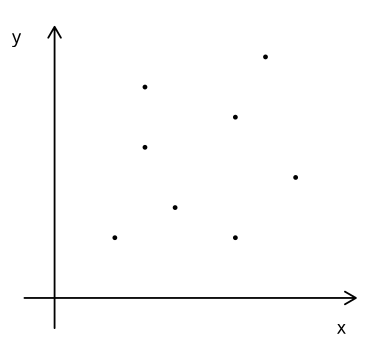
\includegraphics[scale=0.325]{img/scatterplot.png}
    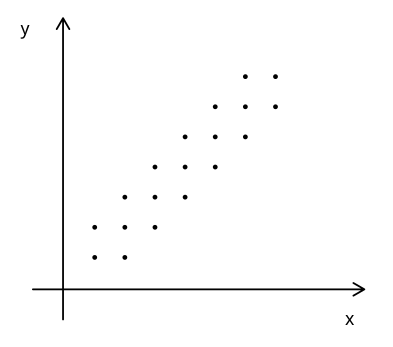
\includegraphics[scale=0.325]{img/scatterplotLineare.png}
    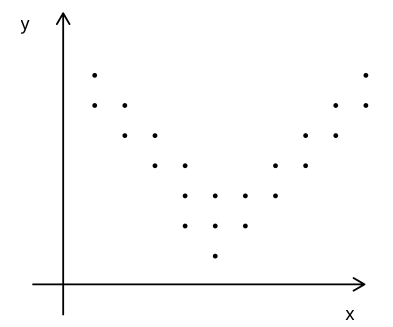
\includegraphics[scale=0.325]{img/scatterplotNonLineare.png}
    \caption{Da sinistra verso destra: Scatterplot Generico, Scatterplot Relazione Lineare, Scatterplot Relazione Non Lineare}
\end{figure}

\paragraph{Regressione} Dato un insieme di punti $(x_{i}, y_{i})$ come possiamo determinare quale curva nel piano approssima meglio quell'insieme? Ci occuperemo solo di
relazioni lineari, la cui classe di curve corrisponde alle rette.

\subsubsection{Covarianza e Correlazioni Campionarie}

Definiamo prima la notazione necessaria:

\[ \boxed{\overline{x} = \frac{1}{n} \sum^{n}_{i=1} x_{i}} \:\:\:\:\:\: \boxed{Var(x) = \frac{1}{n-1}\sum_{i=1}^{n} (x_{i} - \overline{x})} \:\:\:\:\:\: \boxed{\sigma(x) = \sqrt{Var(x)}} \]

\[ \boxed{\overline{y} = \frac{1}{n} \sum^{n}_{i=1} y_{i}} \:\:\:\:\:\: \boxed{Var(y) = \frac{1}{n-1}\sum_{i=1}^{n} (y_{i} - \overline{y})} \:\:\:\:\:\: \boxed{\sigma(y) = \sqrt{Var(y)}} \]

\newpage

\paragraph{Covarianza Campionaria Empirica tra x ed y}

\[ Cov_{e}(x) = \frac{1}{n} \sum^{n}_{i=1} (x_{i} - \overline{x}) (y_{i} - \overline{y}) \]

\[ Cov(x) = \frac{n}{n-1}Cov_{e}(x,y) \]

\paragraph{Coefficiente di Correlazione Campionario tra x e y} Supponiamo $\sigma(x) \neq 0$ e $\sigma(y) \neq 0$ allora:

\vspace*{8px}

\[ r(x,y) = \frac{Cov(x,y)}{\sigma(x) \: \sigma(y)} \]

\subsubsection{Th. Retta di Regressione ai Minimi Quadrati}

Vogliamo trovare la retta di equazione $y=a+bx$ che meglio approssima un insieme di dati bivariati $(x_{i}, y_{i})$. Risulta quindi necessario trovare $a$ e $b$ in modo tale da minimizzare

\[ min_{a,b \in \mathbb{R}} \sum^{n}_{i=1} (y_{i} - (a+bx_{i}) )^{2} \]

\begin{figure}[htbp]
    \center
    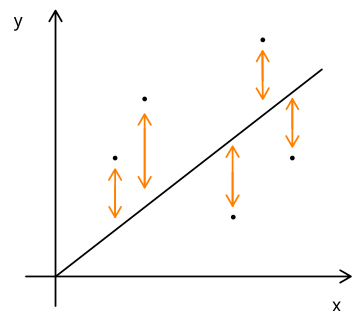
\includegraphics[scale=0.425]{img/teorema-quadrati.png}
\end{figure}

\paragraph{Teorema} Ricaviamo dunque $a,b$ della funzione $y=ax+b$:

\[ b = b^{*} = \frac{Cov(x,y)}{Var{x}} \:\:\:\:\:\: a = a^{*} = \overline{y} - b^{*}\overline{x} \]

\vspace*{5px}

Dunque sostituendo nella funzione da minimizzare definita sopra:

\[ min_{a,b \in \mathbb{R}} \sum^{n}_{i=1} (y_{i} - (a+bx_{i}) )^{2} = \sum^{n}_{i=1} (y_{i} - \overline{y})^{2} (1-r(x,y)^{2}) \]

La retta di regressione è quindi la retta che meglio approssima l'insieme di dati bivariati, la bontà dell'approssimazione lineare è tanto migliore tanto è più piccolo $1-r^{2}$.

\newpage

\section{Probabilità}

Elenchiamo delle definizioni fondamentali per lo studio delle probabilità, ossia la descrizione degli esiti di un esperimento aleatorio:

\begin{enumerate}
    \item \textbf{Spazio Campionario}: Insieme $\Omega$ di tutti i possibili esiti dell'esperimento.
    \item \textbf{Esperimento Aleatorio}: Fenomeno il cui esito non è determinato con certezza a priori.
    \item \textbf{Evento}: Sottoinsieme dello Spazio Campionario, rappresentano \textbf{affermazioni} 
    
    sull'\textbf{esito} dell'\textbf{esperimento}.
    \[ \Omega = \{ 1,2,3,4,5,6 \} \: \: \: \: \text{"Esce numero pari"} = A = \{ 2,4,6 \} \]
    \item \textbf{Relazioni logiche ed operazioni insiemistiche}: Elenchiamo alcune delle operazioni eseguibili:
    \begin{enumerate}
        \item $\text{Accade A o B} \: \mapsto \: A \cup B$
        \item $\text{Accade A e B} \: \mapsto \: A \cap B$
        \item $\text{Non accade A} \: \mapsto \: \overline{A} = \Omega - A$
        \item $\text{Accade A ma non B} \: \mapsto \: A - B$
        \item $\text{Se accade A allora accade B} \: \mapsto \: A \subseteq B$
        \item $\text{A e B non possono accadere contemporaneamente} \: \mapsto \: A \cap B = \varnothing$ 
    \end{enumerate}
    \item \textbf{Definizioni Storiche di Probabilità}: Esistono diverse interpretazioni di probabilità:
    \begin{enumerate}
        \item \textbf{Definizione Classica}: Viene così definita:
        \[ P(A) = \frac{\text{casi favorevoli ad A}}{\text{casi possibili}} = \frac{\#A}{\#\Omega} \]
        \item \textbf{Definizione Frequentista}: Viene così definita:
        \[ P(A) = lim_{n\rightarrow\infty} \: (\text{frequenza relativa di A in n prove ripetute dell'esperimento}) \]
        \item \textbf{Definizione Soggettivista}: Viene così definita:
        \[ P(A) = \text{grado di fiducia che accada A da parte di un soggetto razionale} \]
    \end{enumerate}
\end{enumerate}

L'obiettivo è dunque quello di associare un valore $P(A) \in [0,1]$ ad un evento in modo tale da esprimere quanto sia probabile l'evento $A$ in questione.

\newpage

\paragraph{Regole Fondamentali di Probabilità} Abbiamo visto che esistono varie interpretazioni di probabilità, di conseguenza risulta necessario trovare dei principi minimi che devono essere rispettati
per definire una probabilità. Assumiamo un $\Omega$ spazio campionario ed una funzione $P:\mathbb{P}(\Omega) \rightarrow \mathbb{R}$ dove $\mathbb{P}(\Omega)$ rappresenta l'insieme delle parti di $\Omega$:

\begin{enumerate}
    \item $0 \leq P(A) \leq 1 \:\:\:\:\:\: \forall A \subseteq \Omega$
    \item $P(\Omega) = 1$
    \item Se $A_{i}$ è una successione di eventi a due a due disgiunti (ossia $A_{i} \cap A_{j} = \varnothing \:\: \forall i \neq j$) allora:
    \vspace*{5px}
    \[ P(A_{1} \cup A_{2} \cup \: ... \: \cup A_{n}) = \sum_{i=1}^{n} P(A_{i}) \]
\end{enumerate}

Definiamo grazie a questo uno \textbf{spazio di probabilità}, ossia la coppia $(\Omega, P)$.

\paragraph{Evento Trascurabile ed Evento Quasi Certo}: Definiamo due specifici tipi di eventi:

\begin{enumerate}
    \item \textbf{Evento Trascurabile}: $P(A) = 0$.
    \item \textbf{Evento Quasi Certo}: $P(A) = 1$.
\end{enumerate}

\paragraph{Proprietà di Probabilità} Elenchiamo delle proprietà a disposizione di qualunque probabilità:

\begin{enumerate}
    \item $P(\overline{A}) = 1 - P(A)$
    \item $B \subseteq A \Rightarrow P(A-B) = P(A) - P(B)$
    \item Dati $A,B \subseteq \Omega$ non necessariamente disgiunti, allora:
    \[ P(A \cup B) = P(A) + P(B) - P(A \cap B) \]
\end{enumerate}

% stiamo alla 3.2 delle note corso

\subsection{Modello Uniforme}

Un modello uniforme è uno spazio di probabilità $(\Omega, P)$ tale che $\Omega$ è finito ed ogni esito $\omega \in \Omega$ risulta essere equiprobabile, ossia che
$P(\omega)$ risulta essere la stessa per ogni omega.

\paragraph{Probabilità in Modelli} Se $(\Omega, P)$ è un modello uniforme, allora:

\[ P(A) = \frac{\#A}{\#\Omega} \:\:\:\: \forall A \subseteq \Omega \]

\newpage

\subsubsection{Accenno di Combinatoria}

Elenchiamo diversi tipi di sequenze dato un insieme di $n$ oggetti:

\begin{enumerate}
    \item Numero di sequenze ordinate con ripetizione di k oggetti:
    \[ \#\{ (a_{1}, a_{2}, ... , a_{n}) \} \: | \: a_{j} \in \{ 1,2, ..., n \} = n^{k}\]
    \item Numero di sequenze ordinate senza ripetizione di k oggetti:
    \[ \#\{ (a_{1}, a_{2}, ... , a_{n}) \} \: | \: a_{j} \in \{ 1,2, ..., n \} = \frac{n!}{(n-k)!} \]
    \item Numero di sottoinsiemi di $\{ 1,2,3, ... ,n \}$ formati da $k$ elementi $(k \leq n)$:
    \[ \text{numero sottoinsiemi} = \frac{n!}{k!(n-k)!} \]
\end{enumerate}

\subsection{Probabilità Condizionata}

Dato $(\Omega, P)$ spazio di probabilità, $B$ evento non trascurabile, $A$ evento di probabilità condizionata di $A$ dato $B$:

\[ P(A|B) = \frac{P(A|B)}{P(B)} \]

$P(A|B)$ corrisponde dunque alla probabilità che avvenga $A$ sapendo che si verifica $B$.

\subsubsection{Regole Prodotto, Catena, Fattorizzazione della Probab. Condizionata}

Elenchiamo le regole della Probabilità Condizionata:

\begin{enumerate}
    \item \textbf{Regola Prodotto}: $P(A \cap B) = P(A|B) \: P(B)$
    \item \textbf{Regola Catena}: E' possibile applicare la regola del prodotto $n$ volte. In questo modo di definisce la catena.
    \item \textbf{Regola Fattorizzazione}: La probabilità dell'unione dei rami di una rappresentazione ad albero\footnote{Vedi lezione 3.3, 20/02/2025.} corrisponde alla somma delle probabilità dei rami.
\end{enumerate}

\paragraph{Formula di Fattorizzazione}

Definiamo prima un sistema di alternative 

(eventi $B_{1}, B_{2}, ..., B_{n}$) caratterizzato da:

\begin{enumerate}
    \item Eventi a due a due disgiunti.
    \item $\Omega = \bigcup_{i=1}^{n} B_{i} $
    \item $P(B_{i}) > 0 \: \: \: \: \forall i$
\end{enumerate}

Date quindi $B_{1}, B_{2}, ..., B_{n}$ sistema di alternative, allora $\forall A \subseteq \Omega$:
\vspace*{-5px}
\[ \boxed{P(A) = \sum_{i=1}^{n} P(A|B_{i}) \: P(B_{i}) }\]

\newpage

\subsection{Formula di Bayes}

Siano $A$ e $B$ eventi non trascurabili, allora:

\[ P(B|A) = \frac{P(A|B)\:P(B)}{P(A)} \]

In particolare se $B_{1}, B_{2}, ..., B_{n}$ sistema di alternative, allora:

\[ P(B_{i}|A) = \frac{P(A|B_{i})\:P(B_{i})}{\sum_{j=1}^{n} P(A|B_{j})\:P(B_{j}) } \:\:\:\: \forall i = 1, ..., n \]

\paragraph{Applicazione e Funzionamento}: Solitamente questo teorema viene utilizzato per invertire il condizionamento, tipicamente in due casi:

\begin{enumerate}
    \item Accade un evento $A$ riferito ad un osservabile.
    \item Vogliamo calcolare la probabilità di una possibile causa $B_{i}$.
\end{enumerate}

\subsection{Indipendenza}

Vogliamo definire formalmente in concetto che la probabilità di un determinato evento $A$ non cambia sapendo che accade $B$. Per $A$ e $B$ non trascurabili accade:

\[ P(A) = P(A|B) = \frac{P(A \cap B)}{P(B)} \: \: \Longleftrightarrow \: \: P(A) P(B) = P(A \cap B) \]

Dunque due \textbf{eventi} sono detti \textbf{indipendenti}\footnote{Se due eventi sono disgiunti, allora non sono indipendenti, dato che se accade ad esempio il primo allora non può accadere il secondo.} se:

\[ P(A \cap B) = P(A) \: P(B) \]

\paragraph{Indipendenza a 3 o più Eventi} Dati tre eventi $A,B,C$ questi sono indipendenti se:

\begin{enumerate}
    \item Sono a due a due indipendenti, ossia:
        \[ P(A \cap B) = P(A) \: P(B) ,\:\:\: P(A \cap C) = P(A) \: P(C), \:\:\: P(B \cap C) = P(B) \: P(C) \]
    \item Vale che $P(A \cap B \cap C) = P(A) \: P(B) \: P(C) $
\end{enumerate}

Questo informalmente vuol dire che avere informazioni riguardo alcuni degli eventi non cambia la probabilità relativa degli altri eventi, quindi l'indipendenza a due a due non implica indipendenza globale.

\paragraph{Definizione Indipendenza n-esima Generica} Dati $A_{1}, ..., A_{n}$ eventi indipendenti, la probabilità di ogni possibile intersezione è
il prodotto delle probabilità degli $A_{i}$ coinvolti nell'intersezione:

\vspace{-15px}

\[ P(A_{i1} \cap A_{i2} \: \cap ... \cap \: A_{ik}) = P(A_{i1}) \: P(A_{i2}) \: ... \: P(A_{ik}) \:\:\:\:\: \forall k \leq n, \:\: \forall 1 \leq i_{1} \leq i_{2} \leq ... \leq i_{k} \leq n  \]

\newpage

\subsubsection{Schema di Bernoulli}

Date $n$ prove ripetute, in cui ciascuna prova può avere successo o insuccesso, la formulazione viene così definita:

\[ \Omega = \{ (w_{1}, w_{2}, ..., w_{n}) \: | \: w_{i} \in \{0,1\} \} = \{0,1\}^{n} \]

\[ f = \text{probabilità del successo della singola prova} \]

\vspace{-15px}

\[ P\{ (w_{1}, w_{2}, ..., w_{n}) \} = f^{\#successi} \: (1-f)^{\#insuccessi} = f^{\sum_{i=1}^{n}w_{i}} \: (1-f)^{n - \sum_{i=1}^{n}w_{i}} \]

Da questo possiamo osservare che l'indipendenza non implica l'assenza di causalità e viceversa.

\section{Variabili Aleatorie}

Elenchiamo delle definizioni base:

\begin{enumerate}
    \item \textbf{Variabile Aleatoria (v.a)}: Carattere quantitativo dell'esperimento in esame. Ad esempio in $n$ lanci di moneta $X=\#teste$.
    Nello specifico la definiamo come una funzione $X:\Omega \Rightarrow \mathbb{R}$.
    \item \textbf{Legge/Distribuzione di X}: Distribuzione di probabilità della caratteristica $X$ in esame:
    \[ P^{X}(A) = P(X \in A) = P(\#\text{teste in A}) \:\:\:\: A \subseteq \{0,1, ...,n\} \]
    Nello specifico possiamo anche definirla come probabilità $P^{X}$ su $\mathbb{R}$ data da 
    \[ \{\omega \in \Omega \:|\: X(\omega) \in A\} \]
    \item \textbf{Equidistribuzione}: Due variabili aleatore $X$ ed $Y$ sono dette equidistribuite se \[P^{X} = P^{Y}\].
\end{enumerate}

\subsection{Variabili Aleatorie Discrete}

Una variabile aleatoria $X$ è detta \textbf{discreta} se può assumere un numero finito o numerabile di modalità. Ad esempio nei lanci di moneta, se
\[ X = \text{teste di n lanci di moneta}, \:\:\:\: \text{modalità} = \{ 0,1,2, ..., n \} \]
Questo è un esempio di \textbf{variabile discreta}. Risulta necessario ricordare che parliamo di possibili modalità e non di dati di uno specifico campione.

\newpage

\paragraph{Funzione di Massa (Densità Discreta)}

Data una variabile aleatoria $X$ definiamo $p{X}: \{ a_{1}, a_{2}, ..., a_{n} \} \rightarrow \mathbb{R} $ definita da:

\[ p^{X}(a_{i}) = P\{ X = a_{i} \} = P^{X}(\{a_{i}\}) \]

Da questo possiamo ricavare un altra caratteristica:

\subparagraph{Calcolo delle Probabilità Relative ad X} Dagli statement definiti sopra otteniamo:

\[ P(X \in A) = \sum_{a_{i}\in A} P(X=a_{i}) \]

\subparagraph{Proprietà delle Funzioni di Massa} Data una funzione di massa $p^{X}$, vale che:

\begin{enumerate}
    \item $p^{X}(a_{i}) \geq 0 \:\:\:\: \forall a_{i} $
    \item $\sum_{i}p^{X}(a_{i}) = 1$
\end{enumerate}

Viceversa, se una funzione q soddisfa queste due proprietà allora esiste una variabile aleatoria $X$ che ha $q$ come funzione di massa, e la legge di $X$
è determinata univocamente da $q=p^{X}$.

\subparagraph{Interpretazione delle Definizioni Date} Mostriamo un esempio di estrazione da una popolazione, elencando tutti gli elementi in analisi:

\begin{enumerate}
    \item $\Omega = \{ \text{popolazione} \} $, assumiamo di avere $P$ uniforme, dunque ad \\ esempio $\Omega = \{ \text{italiani} \}, \: X = \#figli $
    \item $X(\omega) = \text{carattere quantitativo di} \:\: \omega$.
    \item $p^{X}(a_{i}) = P(X=a_{i}) = \frac{\#\{ \text{individui con} \: \: X = a_{i} \}}{\#\text{popolazione}} = $ frequenza relativa di  $ \{ X = a_{i} \} $ \\ su tutta la popolazione.
\end{enumerate}

\subsection{Variabili Aleatorie Notevoli}

Questo sottocapitolo elencherà specifiche variabili aleatorie caratterizzate da funzioni di massa predefinite.

Elenchiamo alcune variabili aleatorie notevoli\footnote{Capitoli 4.3, 4.4 delle note del corso 24/25.}:

\begin{enumerate}
    \item \textbf{Variabile Aleatoria Binomiale}: Variabile Aleatoria Discreta di parametri $n \in \mathbb{N^{+}}$, $f \in [0,1]$ con funzione di massa data da:
    \[ p^{X}(k) = P(X=k) = \left (\begin{array}{c} x \\ y \end{array} \right ) f^{k}(1-f)^{n-k} \:\:\:\: k \in \{ 0,1,2, ...,n \} \]


Mostriamo un esempio di utilizzo a pagina successiva.

\newpage

Singola prova: lancio di dado, $5$ prove ripetute, il successo corrisponde all'esito $"6"$, di conseguenza la probabilità è di $\frac{1}{6}$. Quanto vale
la probabilità che almeno due lanci siano uguali a $"6"$?

\[ P(\text{almeno 2 lanci "6"}) = P(X \geq 2 ) = 1 - P(X < 2) = \]

\[ =  1 - P(X=0) - P(X=1) = \]

\[ = 1 - \left (\begin{array}{c} 5 \\ 0 \end{array} \right ) \: \left (\frac{1}{6} \right )^{0} \: \left (1 - \frac{1}{6} \right )^{5-0} - \left (\begin{array}{c} 5 \\ 1 \end{array} \right ) \: \left (\frac{1}{6} \right )^{1} \: \left (1 - \frac{1}{6} \right )^{5-1} \: ... \]

\item \textbf{Variabile Aleatoria Geometrica}: Variabile Aleatoria Geometrica di parametro $p$ con funzione di massa:

\[ p^{T}(k) = \]

\vspace*{-20px}

\[ = f(1-f)^{k-1}, \:\:\: \text{dove} \:\:\: T \:\:\: (\text{istante}) = \text{num. prova primo successo} = min\{ x \in \mathbb{N}^{+} \: | \: \omega_{n} = 1 \} \]

\item \textbf{Variabile Aleatoria Poisson}: $X$ Variabile Aleatoria di Poisson ($Poisson(\lambda)$) di parametro $\lambda > 0$: variabile discreta, a valori
a valori in $\mathbb{N} = \{ 0,1,2, ... \}$, con funzione di massa:

\[ p^{X}(k) = p\{ X = k \} = \frac{\lambda^{k}}{k!}e^{-k} \]

\paragraph{Interpretazione} La variabile aleatoria $X$ di Poisson conta il numero di eventi rari, ossia in numero di successi in $n$ prove ripetute con $n$
molto grande ed $f$ probabilità di successo molto piccola (ossia in successo è raro), con $\lambda = nf > 0$.

\end{enumerate}

\subsection{Variabili Aleatorie con Densità}

Le variabili aleatorie $X$ con densità sono caratterizzate appunto da una funzione $f:\mathbb{R} \rightarrow \mathbb{R}$ dove $P(X)$ corrisponde a:

\[ P(X \in A) = \int_{A} f(x)dx \]

Quindi $P(X)$ corrisponde all'area sottesa alla funzione. Questo implica che ogni caratteristica sugli estremi dell'integrale influenzerà la densità ed il suo calcolo.

\paragraph{Interpretazione} La densità calcolata sulla funzione $f$ corrisponde alla distribuzione di $X$ per unità di lunghezza. Questo tipo di variabili si utilizzano per caratteri continui.

\newpage

\paragraph{Proprietà delle Densità} Elenchiamo le proprietà delle densità:

\begin{enumerate}
    \item $f(x) \leq 0 \:\:\:\:\: \forall x \in \mathbb{R} $
    \item $\int_{+\infty}^{-\infty} f(x)dx = 1$
\end{enumerate}

Di conseguenza se $f$ soddisfa le due proprietà allora esiste almeno una variabile aleatoria $X$ con densità $f$ e la sua distribuizione è
univocamente determinata da $f$. 

\subsubsection{Variabili Aleatorie con Densità Note}

Elenchiamo e descriviamo alcune variabili con densità note:

\begin{enumerate}
    \item \textbf{Variabili Aleatorie Uniformi}: $X$ variabile uniforme su un intervallo $(\alpha, \beta)$ dato $(U(\alpha, \beta))$ con densità:
    \[ f(x) =  \left\{ \begin{array}{rcl}
        \frac{1}{\beta - \alpha} & \mbox{se} & x \in (\alpha,\beta) \\
         0 & \mbox{se} & x \notin (\alpha,\beta)
        \end{array}\right. \]
    La parte a tratti viene "fattorizzata" come un ulteriore funzione, ossia:
    \[ {1}_{A}(x) =  \left\{ \begin{array}{rcl}
        {1} & \mbox{se} & x \in (\alpha,\beta) \\
         0 & \mbox{se} & x \notin (\alpha,\beta)
        \end{array}\right. \]
    Di conseguenza la funzione viene così definita:
    \[ f(x) = \frac{1}{\beta - \alpha} \: 1_{\alpha, \beta}(x) \]
    \paragraph{Interpretazione} Viene scelto un punto a caso nell'intervallo dato senza alcuna preferenza.

    \item \textbf{Variabili Aleatorie Esponenziali}: $X$ variabile esponenziale di parametro $\lambda > 0$ e con densità:
    \vspace*{15px}
    \[ f(x) =  \left\{ \begin{array}{rcl}
        \lambda e^{-\lambda x} & \mbox{se} & x > 0 \\
         0 & \mbox{se} & x \leq 0
        \end{array}\right. \]
    Fattorizzando con la funzione $1(x)$ vista prima otteniamo $f(x) = \lambda e^{-\lambda x}\: 1_{0,+\infty}(x) $. 
    \paragraph{Interpretazione} Tempo di attesa tra due eventi rari.
\end{enumerate}

\newpage

\subsection{Funzione di Ripartizione e Quantili}

Data $X: \Omega \rightarrow \mathbb{R}$ variabile aleatoria, $P_{X}$ legge di $X$ e $P_{X}(A) = P(X \in A)$ con $A \in \mathbb{R}$, definiamo la funzione
di ripartizione (FdR) di $X$ con:

\[ F_{X}: \mathbb{R} \rightarrow [0,1] \: \: \text{data da} \: \: F_{X}(x) = P(X \leq x) = P_{X}((-\infty, x]), \:\:\: x \in \mathbb{R}  \]

\paragraph{Proprietà di FdR} Elenchiamo le proprieta della funzione di ripartizione:

\begin{enumerate}
    \item Non decrescente.
    \item Continua a destra.
    \item $lim_{x \rightarrow +\infty} F(x) = 1, \:\: lim_{x \rightarrow -\infty} F(x) = 0 $
\end{enumerate}

\paragraph{Legame tra FdR e Densità} Esiste un legame tra FdR e Densità:

\[ F_{X}(x) = \int_{-\infty}^{x} f(y)dy \]

Questo accade se $F_{X}$ è continua, viceversa se $f$ è continua a tratti:

\[ f(x) = F^{'}_{X}(x) \]

\paragraph{Calcolo Probabilità Intervalli} Calcoliamo la probabilità di un intervallo:

\[ P(a \leq X \leq b) = F_{X}(b) - F_{X}(a) \]

\subparagraph{Probabilità e Beta-Quantili} Data $X$ variabile aleatoria, dato $\beta \in (0,1)$ allora $\beta-$quantile:

\[ \text{numero } r_{\beta} \text{ tale che } P(X \leq r_{\beta}) \geq \beta \: \: \text{e} \: \: \: \: P(X \geq r_{\beta}) \geq 1 - \beta \]

\newpage

\subsection{Variabili Aleatorie Gaussiane}

Definiamo $Z$ o $N(0,1)$ variabile gaussiana (o normale) standard, nello specifico corrisponde ad una variabile aleatoria con densità:

\[ y(x) = \frac{1}{\sqrt{2\pi}}e^{\frac{-x^{2}}{2}} \]

\paragraph{Funzione di Ripartizione e Beta Quantili di N}

\[ \Phi(x) = P(Z \leq x) = \int_{x}^{-\infty} \frac{1}{\sqrt{2\pi}} e^{\frac{-y^{2}}{2}} dy \:\:\:\: (\text{FdR})\]

\[ q_{\beta} = \Phi^{-1}(\beta) \:\:\:\: (\text{Beta-Quantile})\]

\paragraph{Esempio di Utilizzo FdR} Mostriamo un esempio in cui risulta necessario utilizzare la FdR:

\begin{enumerate}
    \item Immaginiamo di voler calcolare questa probabilità:
    \[ P(a < z < b) = \int_{a}^{b} y(x)dx \]
    Non esiste un espressione esplicita per questo integrale.
    \item Si usa allora la FdR:
    \[ P(a < z < b) = \Phi(b) - \Phi(a) \]
\end{enumerate}

\subsubsection{Trasformazioni di Variabili Aleatorie con Densità}

Data $X:\Omega \rightarrow \mathbb{R}$ ed $h:\mathbb{R} \rightarrow \mathbb{R}$ allora $h \: o \:X : \Omega \rightarrow \mathbb{R}$ è anch'essa una variabile
aleatoria. Ma $h \: o \:X$ ammette densità? In generale no, ammette densità solo se $h$ è invertibile.

\paragraph{*** Proposizione sul cambio di variabile ***}

\subsubsection{Variabile Aleatoria Gaussiana Generale}

Dati $Z = N(0,1)$, $m \in \mathbb{R}$, $\sigma > 0$, $Y=h(z)=\sigma Z + m$ con densità:

\[ f(y) = \frac{1}{\sigma}y(\frac{y-m}{\sigma}) = \frac{1}{\sqrt{2 \pi \sigma^{2}}} \: exp \left( -\frac{(y-m)^{2}}{2 \sigma^{2}} \right) \]

\paragraph{Definizione} $Y$ variabile aleatoria gaussiana di media $m$ e varianza $\sigma^{2}$ con densità:

\[ f(y) = \frac{1}{\sqrt{2 \pi \sigma^{2}}} \: exp \left( -\frac{(y-m)^{2}}{2 \sigma^{2}} \right) \:\:\:\: y \in \mathbb{R} \]

In generale dunque ci riferiremo a questo tipo di variabile aleatoria con $(N(m,\sigma^{2}))$.

\newpage

\paragraph{Standardizzazione tra due tipi di N}

Dato $(N(m,\sigma^{2}))$ possiamo dirigerci verso $Z = N(0,1)$ tramite standardizzazione:

\[ Z = N(0,1) \Leftrightarrow y = \sigma Z + m  = N(m, \sigma^{2}) \:\:\: \text{quindi}\]

\[ P(a < Y < b) = P(\frac{a-m}{\sigma} < Z < \frac{b-m}{\sigma}) = \Phi \left( \frac{b-m}{\sigma} \right)- \Phi\left(\frac{a-m}{\sigma} \right) \:\:\:\: (\Phi \:\: \text{FdR di} \: \: N(0,1)) \]

\subsection{Valore Atteso e Momenti}

Data $X$ variabile aleatoria \textbf{discreta}, a valori in $a_{1}, a_{2}, ...$, con funzione di massa $p$ il valore atteso di $X$:

\[ \mathbb{E}[X] = \sum_{j} a_{j}\: p(a_{j}) \]

\paragraph{Interpretazione}

Può essere visto come il baricentro di $P$, o la media delle $a_{j}$ pesata con $p(a_{j})$. E' dunque la media su tutta la popolazione e non su un singolo campione.

\paragraph{Valore Atteso su Variabile Aleatoria con Densità} Data $X$ variabile aleatoria con densità $f$, il valore atteso di $X$:

\[ \mathbb{E}[X] = \int_{+\infty}^{-\infty} x\:f(x) dx \]

Il valore atteso in queste condizioni non è sempre finito, di conseguenza non è sempre definito. Quando è definito:

\begin{enumerate}
    \item Se $X$ variabile aleatoria (discreta o con densità) è $\geq 0$, allora:
    \[ \exists \:\: \mathbb{E}[X] = \sum_{j} a_{j}p(a_{j}) \:\:\: \text{oppure} \:\:\: \int x\:f(x)dx \:\:\:\:\:\: \in [0,+\infty] \]
    \item Per variabile aleatoria generica, $X$ ammette valore atteso se:
    \[ \mathbb{E}[X] = \sum_{j} |a_{j}|\:p(a_{j}) \:\:\: \text{oppure} \:\:\: \int |x|\:f(x)dx \:\:\:\:\:\: < \: +\infty \]
    rispettivamente se è un caso discreto o con densità.
    \item Criteri sufficienti per $\exists \: \mathbb{E}[X] \in \mathbb{R}$:
    \begin{enumerate}
        \item Caso Discreto: Se $a_{j}$ sono in numero finito.
        \item Caso con Densità: Se $f=0$ fuori da un intervallo limitato $[\alpha,\beta]$.
    \end{enumerate}
\end{enumerate}

\newpage

\subsubsection{Calcolo e Proprietà del Valore Atteso}

\paragraph{Calcolo Valore Atteso} Data una variabile aleatoria $X$ discreta o con densità, calcoliamo il valore atteso:

\begin{enumerate}
    \item Se $X$ è discreta con funzione di massa $p$:
    \[ \mathbb{E}[g(X)] = \sum_{j} g(a_{j})\:p(a_{j}) \]
    \item Se $X$ ha densità $f$:
    \vspace*{10px}
    \[ \mathbb{E}[g(X)] = \int_{+\infty}^{+\infty} g(x)\:f(x)\:dx \]
\end{enumerate}

\paragraph{Proprietà Valore Atteso} Siano $X,Y$ variabili aleatorie date e $a,b \in \mathbb{R}$:

\begin{enumerate}
    \item \textbf{Linearità}:
    \begin{enumerate}
        \item $\mathbb{E}[X+Y] = \mathbb{E}[X] + \mathbb{E}[Y]$
        \item $\mathbb{E}[aX+b] = a\mathbb{E}[X] + b$
    \end{enumerate}
    \item \textbf{Monotonia}:
    \begin{enumerate}
        \item Se $X \geq 0$, allora $\mathbb{E}[X] \geq 0$
        \item Se $X \geq Y$, allora $\mathbb{E}[X] \geq \mathbb{E}[Y]$
    \end{enumerate}
\end{enumerate}

\paragraph{Momento di Ordine n-esimo} Data una variabile aleatoria $X$:

\[ \mathbb{E}[X^{n}] =  \left\{ \begin{array}{rcl}
        \sum_{j} a^{n}_{j} \: P(X = a_{j}) & \mbox{caso discreto}  \\
        \int_{-\infty}^{+\infty} x^{n}\: f(x) \: dx   & \mbox{caso con densità} 
        \end{array}\right. \]

\paragraph{Disequazione di Markov}

\vspace*{5px}

Sia X variabile aleatoria $\leq 0,\: a > 0$, allora:

\[ P(X \geq a) \leq \frac{1}{a} \mathbb{E}[X] \]

\subparagraph{Dimostrazione} Dimostriamo la disequazione di Markov:

%\vspace*{10px}

\[ a 1[X] \geq a(\omega) \geq X(\omega) \]
\[ E[a\:1[X \geq a]] \leq E[X] \]
\[ 0 \: P(X < a) + a \: P(X \geq a ) = a \: P(X \geq a) \]

\newpage

\subsection{Varianza e Deviazione Standard}

Riprendendo la varianza empirica:

\[ Var_{e}(x) = \frac{1}{n}\sum_{i=1}^{n} (x_{i} - \overline{x})^{2} = \sum_{j=1}^{m} (a_{j} - \overline{x})^{2} \: * \: \text{frequenza relativa di} \: a_{j}   \]
che rappresenta la dispersione dei dati attorno a $\overline{x}$.

\paragraph{Definizione} Data $X$ variabile aleatoria con momento secondo $(E[X^{2}]  )$, allora la varianza di $X$ sarà:

\[ Var(X) = E[(X- E[X])^{2}] = \sigma(x^{2})\]

La deviazione standard di X invece sarà:

\[ \sigma(X) = \sqrt{Var(X)} \]

\paragraph{Interpretazione della Varianza}

Media degli scarti quadratici da $E[X]$: indice della dispersione di $X$, più grande sarà la dispersione e maggiore sarà in modulo da **.**.

\paragraph{Calcolo della Varianza} Definiamo il calcolo 

\[ Var(X) = E[X^{2}] - E[X]^{2} \]

dove

\[ \sum a^{2}_{j}\: p^{X}(a_{j}) - E[X]^{2} \:\:\:\: \text{Se discreto} \]
\[ \int x^{2}\: f(x)\:dx - E[X]^{2} \:\:\:\: \text{Se con densità}\]

\paragraph{Proprietà di Scaling della Varianza} Immaginiamo $X$ v.a e $a,b \in \mathbb{R}$

\[ Var(aX + b) = a^{2} \: Var(X) \] 

\paragraph{Disequazione di Chebyshev}

Data $X$ v.a con momento secondo, $d > 0$:

\[ P(|X - E[X]| \geq d) \leq \frac{1}{d^{2}}Var(x) \]

Stiamo quindi cercando di capire la probabilità che un valore stia fuori da un intervallo in termini di dispersione.

\newpage

\subsection{Valore Atteso e Varianza per Esempi Notevoli}

\begin{enumerate}
    \item \textbf{Binomiale} $(n,p)$: Conta i numeri di successi in $n$ prove ripetute, con probabilità di successo $p$:
    \[ E[X] = 0 * P(X = 0) + 1 * P(X=1) = p \]
    \[ E[X^{2}] = 0^{2} * P(X = 0) + 1^{2} * P(X=1) = p \]
    \[ Var(X) = p - p^{2} = p(1-p) \]
    \begin{enumerate}
        \item \textbf{n Generica}:
        \[ X_{i} =  \left\{ \begin{array}{rcl}
        1 & \mbox{se successo alla i-esima prova}  \\
        0 & \mbox{altrimenti} 
        \end{array}\right. \]
        \[ X = X_{1} + \cdots + X_{n} =  \]
        \[ E[X] = E[X_{1}] + \cdots + E[X_{n}] = np \]
        \[ Var(X) = np(1-p) \]

    \end{enumerate}
    \item \textbf{Geometrica}: Istante del primo successo è $T$ con $P(T=k) = p(1-p)^{k-1} $
    \[ E[T] = \frac{1}{p} \]
    \[ Var(T) = \frac{1-p}{p^{2}} \]
    \item \textbf{Poisson}: Avendo $P(X=k)=\frac{\lambda^{k}}{k!}e^{-\lambda}$
    \[ E[X] = \lambda \]
    \[ Var(X) = \lambda \]
    \item \textbf{Variabile Uniforme su Intervallo}: Variabile con densità $f(x) = \frac{1}{\beta - \alpha}\:1_{\alpha,\beta}(x)$:
    \[ E[X] = \frac{\alpha + \beta}{2} \]
    \[ E[X] = \int_{\alpha}^{\beta} x \: \frac{1}{\beta - \alpha} dx = \cdots = \frac{\alpha + \beta}{2} \]
    \[ E[X^{2}] = \int_{\alpha}^{\beta} x^{2} \frac{1}{\beta - \alpha} dx = \cdots =  \]
    \[ Var(X) = \frac{(\beta - \alpha)^{2}}{12} \]
    \item \textbf{Esponenziale}: Dato un $\lambda$, avendo una densità $f(x) = \lambda e^{-\lambda x}\:1_{(0,+\infty)}(x)$:
    \[ E[X] = \int_{0}^{\infty} x \lambda e^{-\lambda x} dx = \cdots = -\frac{1}{\lambda}e^{-\lambda x} = \cdots = \frac{1}{\lambda} \]
    \[ Var(X) = \frac{1}{\lambda^{2}} \]
\newpage
    \item \textbf{Normali}: $X = N(m, \sigma^{2})$:
    \[ m = 0, \: \: \sigma = 1 \:\:\:\: Z = N(0,1) \]
    \[ E[Z] = \int_{-\infty}^{\infty} x \frac{1}{\sqrt{2\pi}}e^{\frac{-x^{2}}{2}} dx = 0\]
    \[ E[Z^{2}] = Var(Z) = 1 \]
    In generale però, per standardizzazione:
    \[ X = \sigma Z + m \]
    \[ E[X] = \sigma E[Z] + m = m \:\:\:\: \text{(per Linearità)} \]
    \[ Var(X) = \sigma^{2} Var(Z) = \sigma^{2} \:\:\:\: \text{(per Scaling)}\]

\end{enumerate}

\section{Variabili Aleatorie Multivariate}

Descriviamo le caratteristiche di variabili composte di più di una caratteristica:

\subsection{Variabile Aleatoria Doppia} Dato uno spazio di probabilità $(\Omega, P)$ variabile rappresentata da una coppia $(X,Y)$ che corrisponde ad una funzione $(X,Y): \Omega \rightarrow \mathbb{R}^{2}$
dove \[ \omega \in \Omega \mapsto (X(\omega), Y(\omega)) \in \mathbb{R}^{2} \]

Questa variabile dunque è una coppia di caratteristiche quantitative degli esiti 

dell'esperimento.

\paragraph{Legge Congiunta di (X,Y)} 

\[ P^{(X,Y)}: \mathbb{P}(\mathbb{R}^{2}) \rightarrow \mathbb{R} \:\: \text{data da} \:\: P^{(X,Y)}(C) = P((X,Y) \in C) \:\: \forall C \in \mathbb{R}^{2} \]
\begin{center}
    dove
\end{center}
\[ \{ (X,Y) \in C \} = (X,Y)^{-1} (C) \]

\paragraph{Legge Marginale di X e di Y}

\[ \text{Legge} \: \: P^{X} \: \text{di} \: X: P^{X}(A) = P(X \in A)  \]
\[ \text{Legge} \: \: P^{Y} \: \text{di} \: Y: P^{Y}(B) = P(Y \in B)  \]

\paragraph{Interpretazione della Conguinta/Marginale} La legge congiunta a differenza di quella marginale permette di mantenere informazioni riguardo le possibili
relazioni tra le caratteristiche $X$ ed $Y$. Quindi dalla congiunta sarà possibile ricavare le marginali, ma non il contrario dato che non avremo le informazioni riguardo la relazione nelle marginali.

\newpage

\paragraph{Variabile Doppia Discreta} Una variabile aleatoria doppia è detta discreta se $(X,Y)$ assume un numero finito o numerabile di valori, cioè se $X$ ed $Y$ sono discrete.

\paragraph{Funzione di Massa Congiunta di (X,Y)} Descriviamo la funzione di massa in questo contesto:

\[ p^{(X,Y)}(a,b) = P(X=a,Y=b) \:\:\:\: (a,b) \in \mathbb{R}^{2} \]

Da questa è possibile calcolare la legge congiunta come somma di funzioni di massa appartenenti a $C$:

\[ P((X,Y) \in C) = \sum_{(a,b) \in C} P(X=a, Y=b) \:\:\:\: \forall C \in \mathbb{R}^{2} \]

Definiamo cosa abbiamo prima accennato, ossia la possibilità di poter ricavare le funzioni di massa marginali dalla legge congiunta:

\[ P(X = a) = \sum_{b \in \mathbb{R}} P(X=a, Y=b) \]
\[ P(Y = b) = \sum_{a \in \mathbb{R}} P(X=a, Y=b) \]


\newpage

\end{document}